\documentclass{scrreprt}
\usepackage{listings}
\usepackage{underscore}
\usepackage{graphicx}
\usepackage[a4paper,bindingoffset=0.2in,%
left=0.5in,right=1in,top=0.2in,bottom=0.1in,%
footskip=.25in]{geometry}

\usepackage{courier} %% Sets font for listing as Courier.
\usepackage{listings, xcolor}
\usepackage{courier} %% Sets font for listing as Courier.
\usepackage{listings, xcolor}
\lstset{
	tabsize = 4, %% set tab space width
	showstringspaces = false, %% prevent space marking in strings, string is defined as the text that is generally printed directly to the console
	numbers = left, %% display line numbers on the left
	commentstyle = \color{red}, %% set comment color
	keywordstyle = \color{blue}, %% set keyword color
	stringstyle = \color{red}, %% set string color
	rulecolor = \color{black}, %% set frame color to avoid being affected by text color
	basicstyle = \small \ttfamily , %% set listing font and size
	breaklines = true, %% enable line breaking
	numberstyle = \tiny,
}



\usepackage[bookmarks=true]{hyperref}
\usepackage[utf8]{inputenc}
\usepackage[english]{babel}
\hypersetup{
    bookmarks=false,    % show bookmarks bar?
    pdftitle={Software Requirement Specification},    % title
    pdfauthor={Jean-Philippe Eisenbarth},                     % author
    pdfsubject={TeX and LaTeX},                        % subject of the document
    pdfkeywords={TeX, LaTeX, graphics, images}, % list of keywords
    colorlinks=true,       % false: boxed links; true: colored links
    linkcolor=blue,       % color of internal links
    citecolor=black,       % color of links to bibliography
    filecolor=black,        % color of file links
    urlcolor=purple,        % color of external links
    linktoc=page            % only page is linked
}%
\def\myversion{1.0 }
\date{}
%\title
\usepackage{hyperref}
\begin{document}

\begin{flushright}
    \rule{16cm}{5pt}\vskip1cm
    \begin{bfseries}
        \LARGE{REQUIREMENTS\\ SPECIFICATION}\\
        \vspace{1.5cm}
        for\\
        \vspace{1.5cm}
        ECCD DBMS\\
        \vspace{1.5cm}
        Prepared by : 12190011\\12190004\\12190022\\
        \vspace{1.5cm}
        Submitted to :  Mulualem Teku\\Lecturer\\
        \vspace{1.5cm}
        \today\\
    \end{bfseries}
\end{flushright}


\newpage
\chapter{Requirement Gathering}

	\section{Introduction/Background}
Early Childhood Care and Education is known in Bhutan as Early Childhood Care and Development, ECCD.\\The ECCD, here at Gyelpozhing is known as Kurichuu Early Childhood Care and Development. It is a coorperate ECCD started by the Kurichhu project in August 1, 2010. The ECCD was mainly established for the wellbeing for the children of the employees working in Kurichuu project. 
 

	\section{Vision and Mission}
	Kurichuu Early Childhood Care and Development, vision and mission:\\
"Learn and Play"

	\section{Scope}
The client for our DBMS project we will be Kurichuu Early Childhood Care and Development, in Gyelpozhing, Mongar.  


	\section{Objective}
With this project we will be able to design a database managent system suitable for the ECCD


	\section{Study of Similar Systems}
	\begin{itemize}
		\item Paper-based File System\\System of storing data in paper files, this system started eversince paper was invented. There are small organisations who follow the paper-based file system even today. \\However it is widely held that keeping and maintaining paper-based documents is unnecessarily cumbersome and costly, now that we have the option of maintaining electronic versions of documents.
		
	
		\item Spreadsheet\\The Kurichhu ECCD, follows a paper based file system. Mainly because the organisation is small in number, with four facilitator and 54 children. \\The information regarding the children are maintained in paper-based files as well as in spreedsheet.
		
  		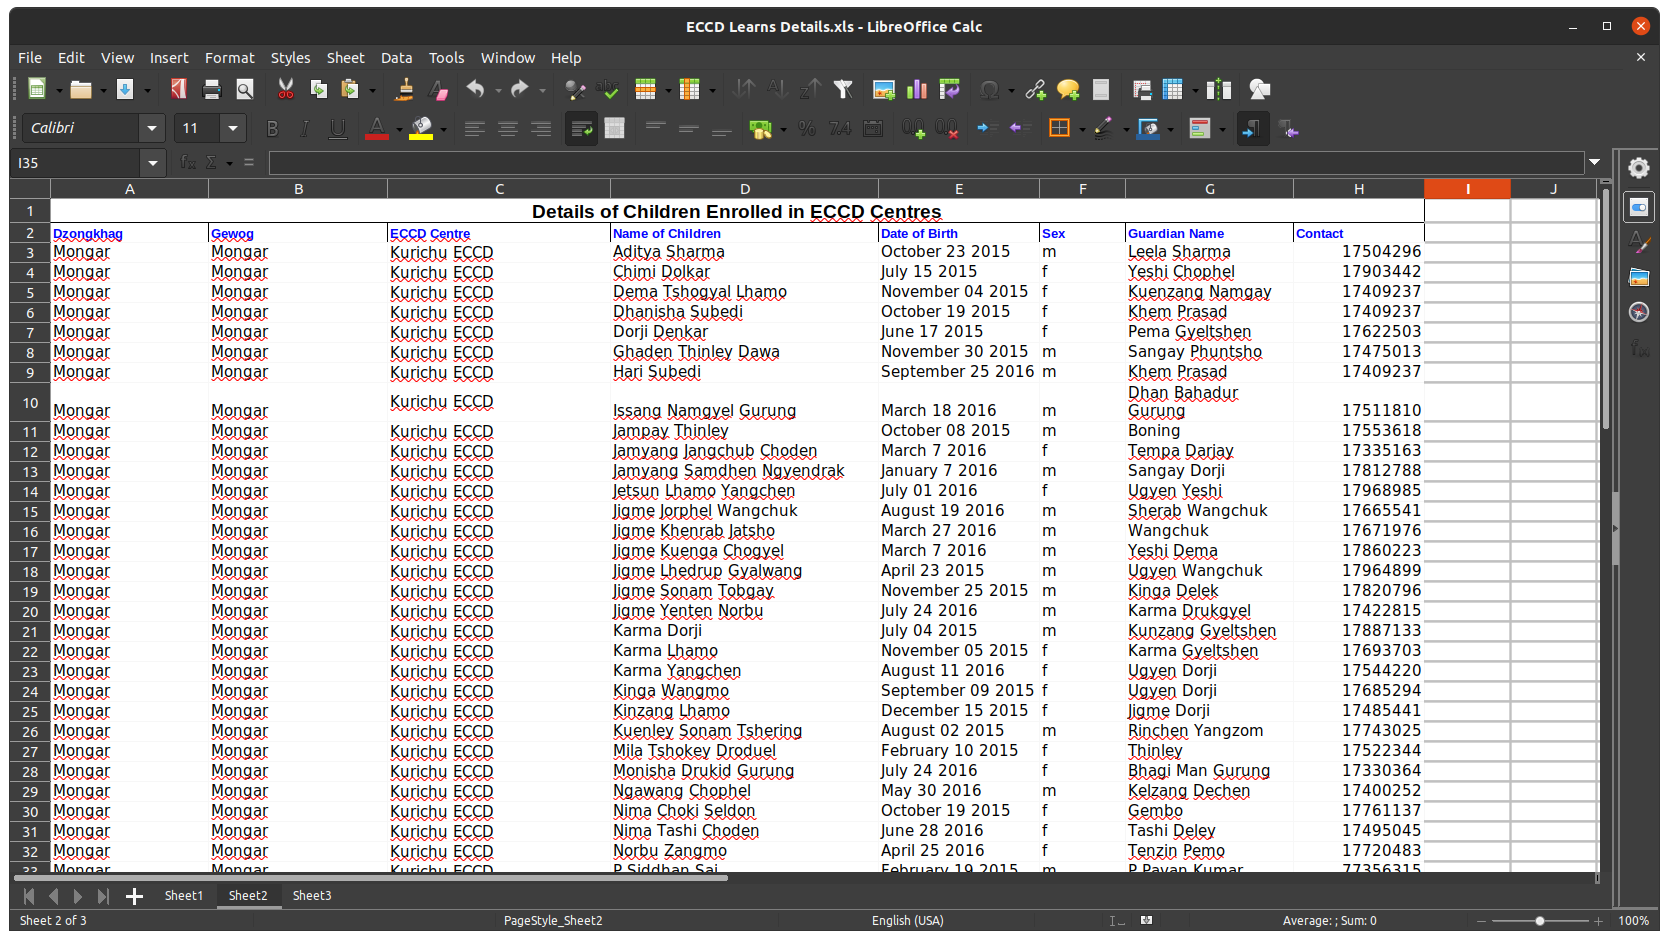
\includegraphics[scale=0.2]{c}
 			
  		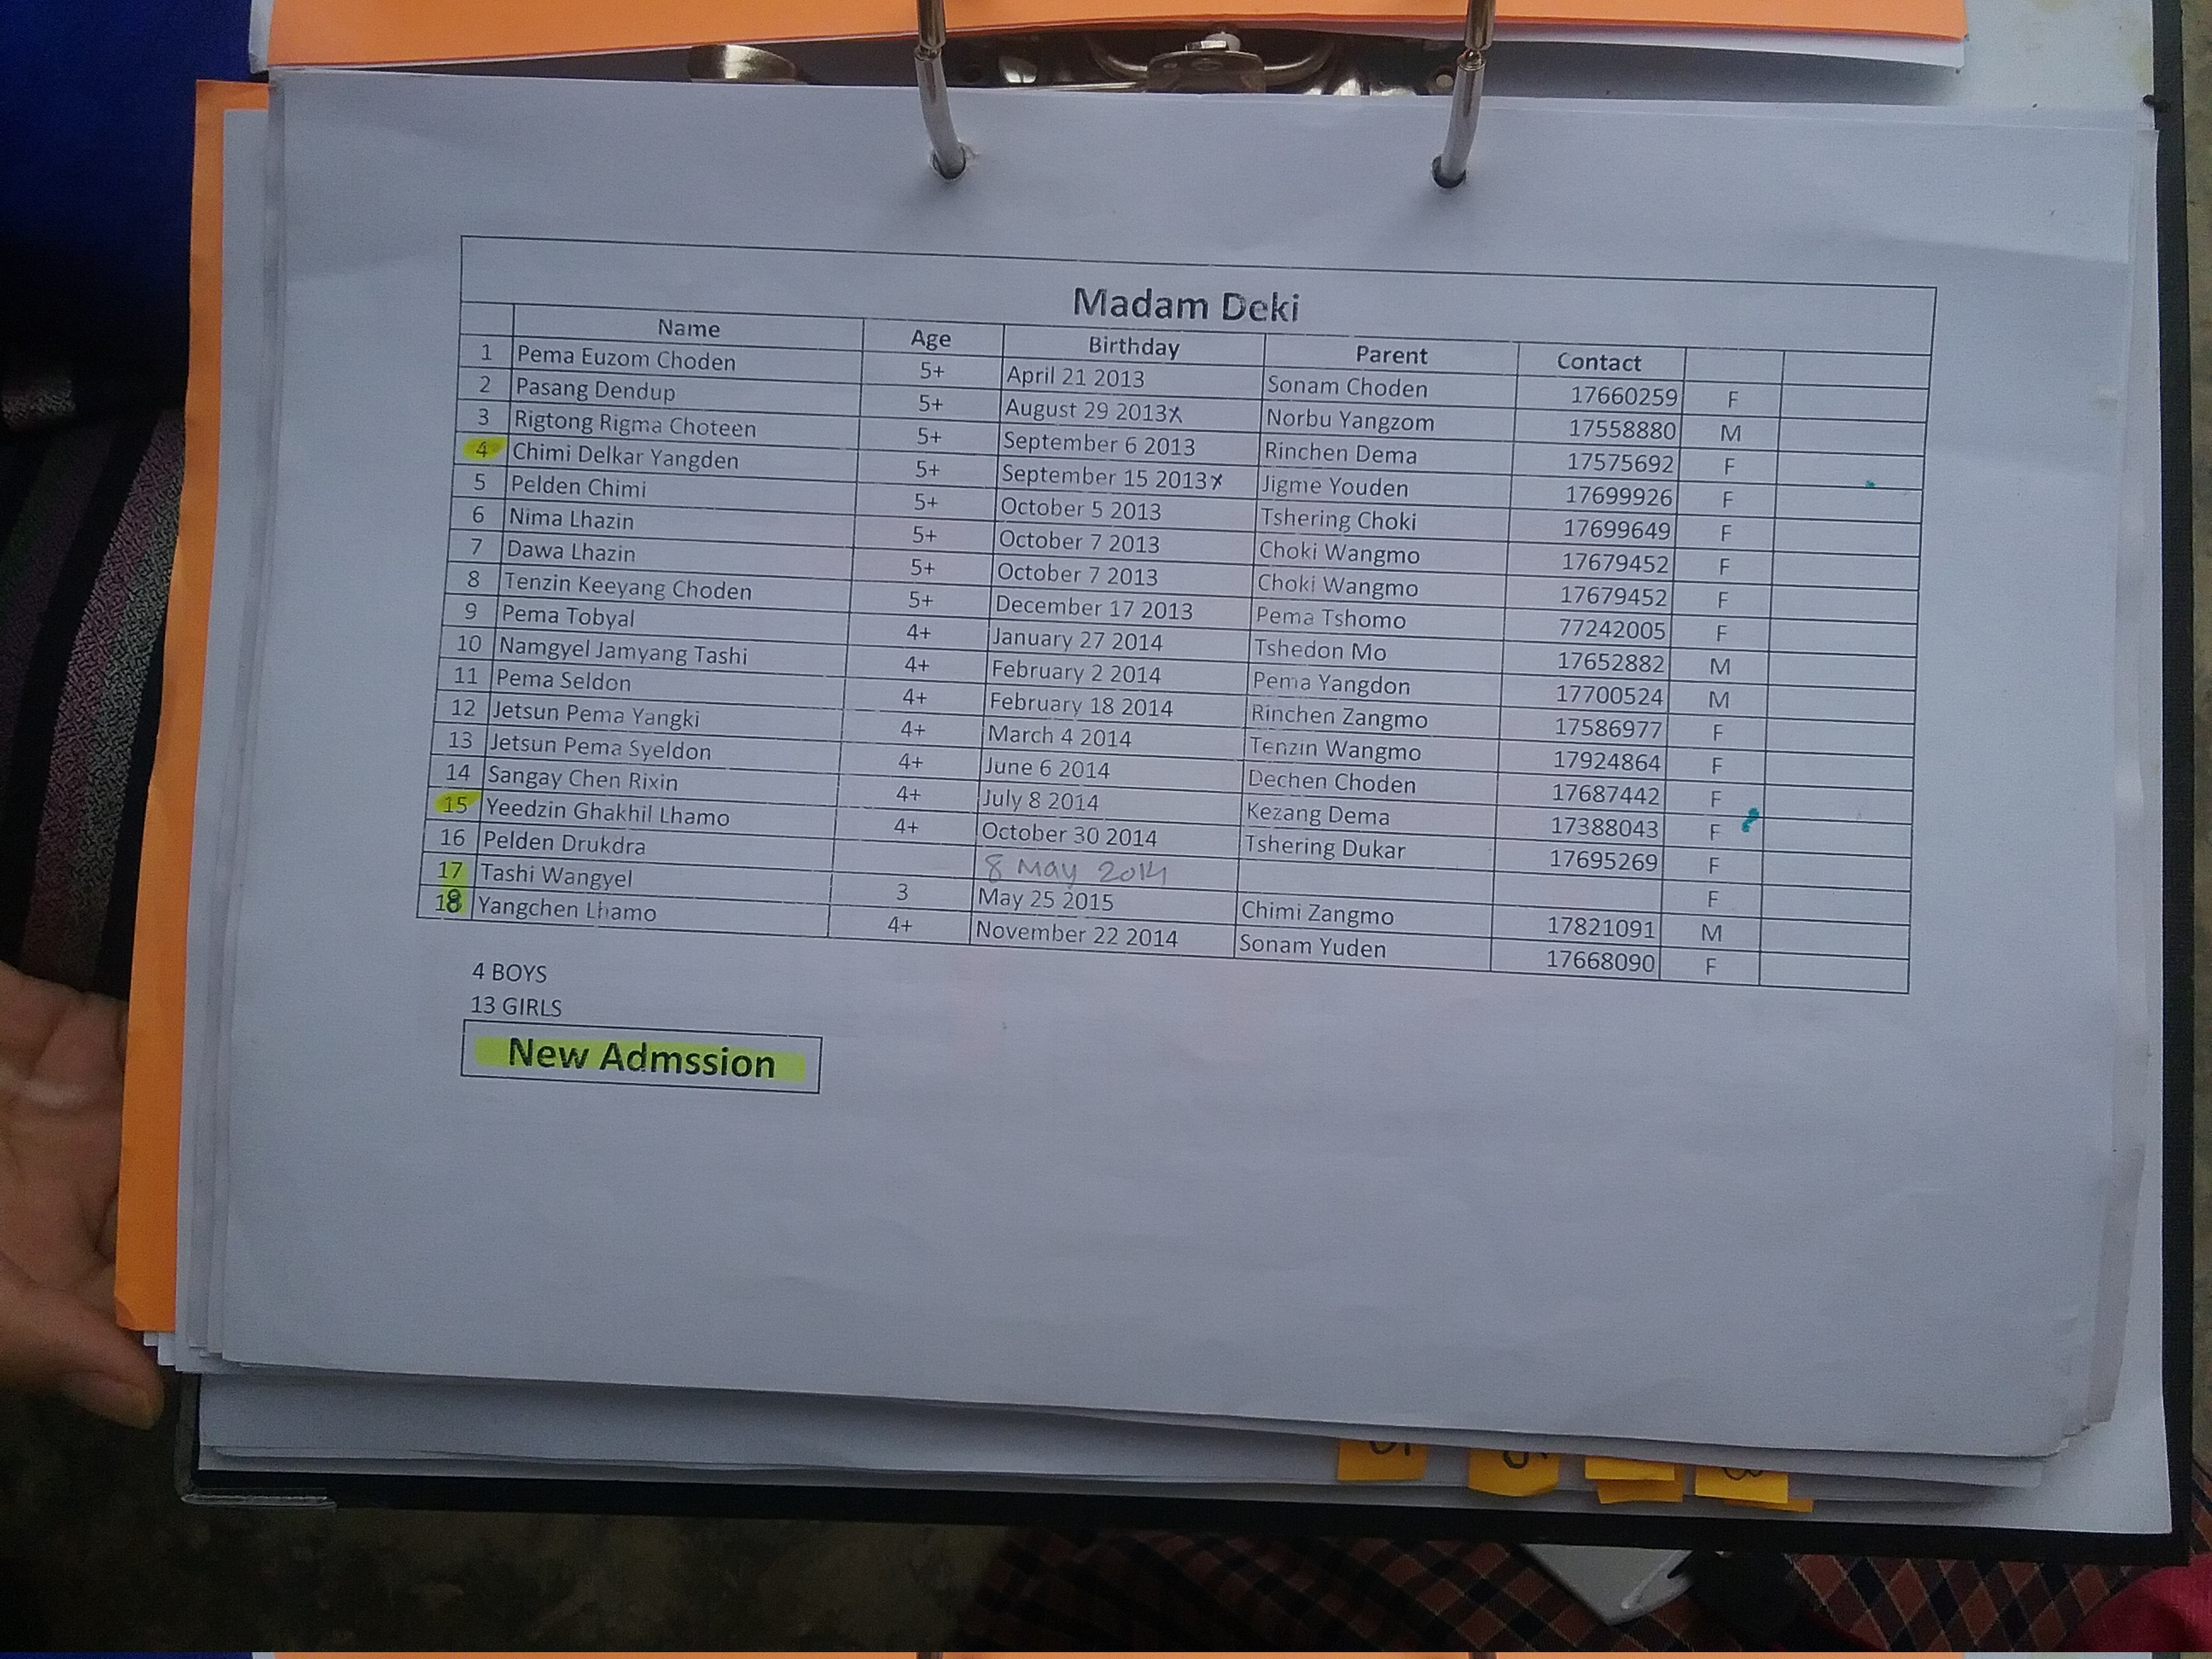
\includegraphics[scale=0.2]{8}
  		
		 For each year they maintain a different file.
		
		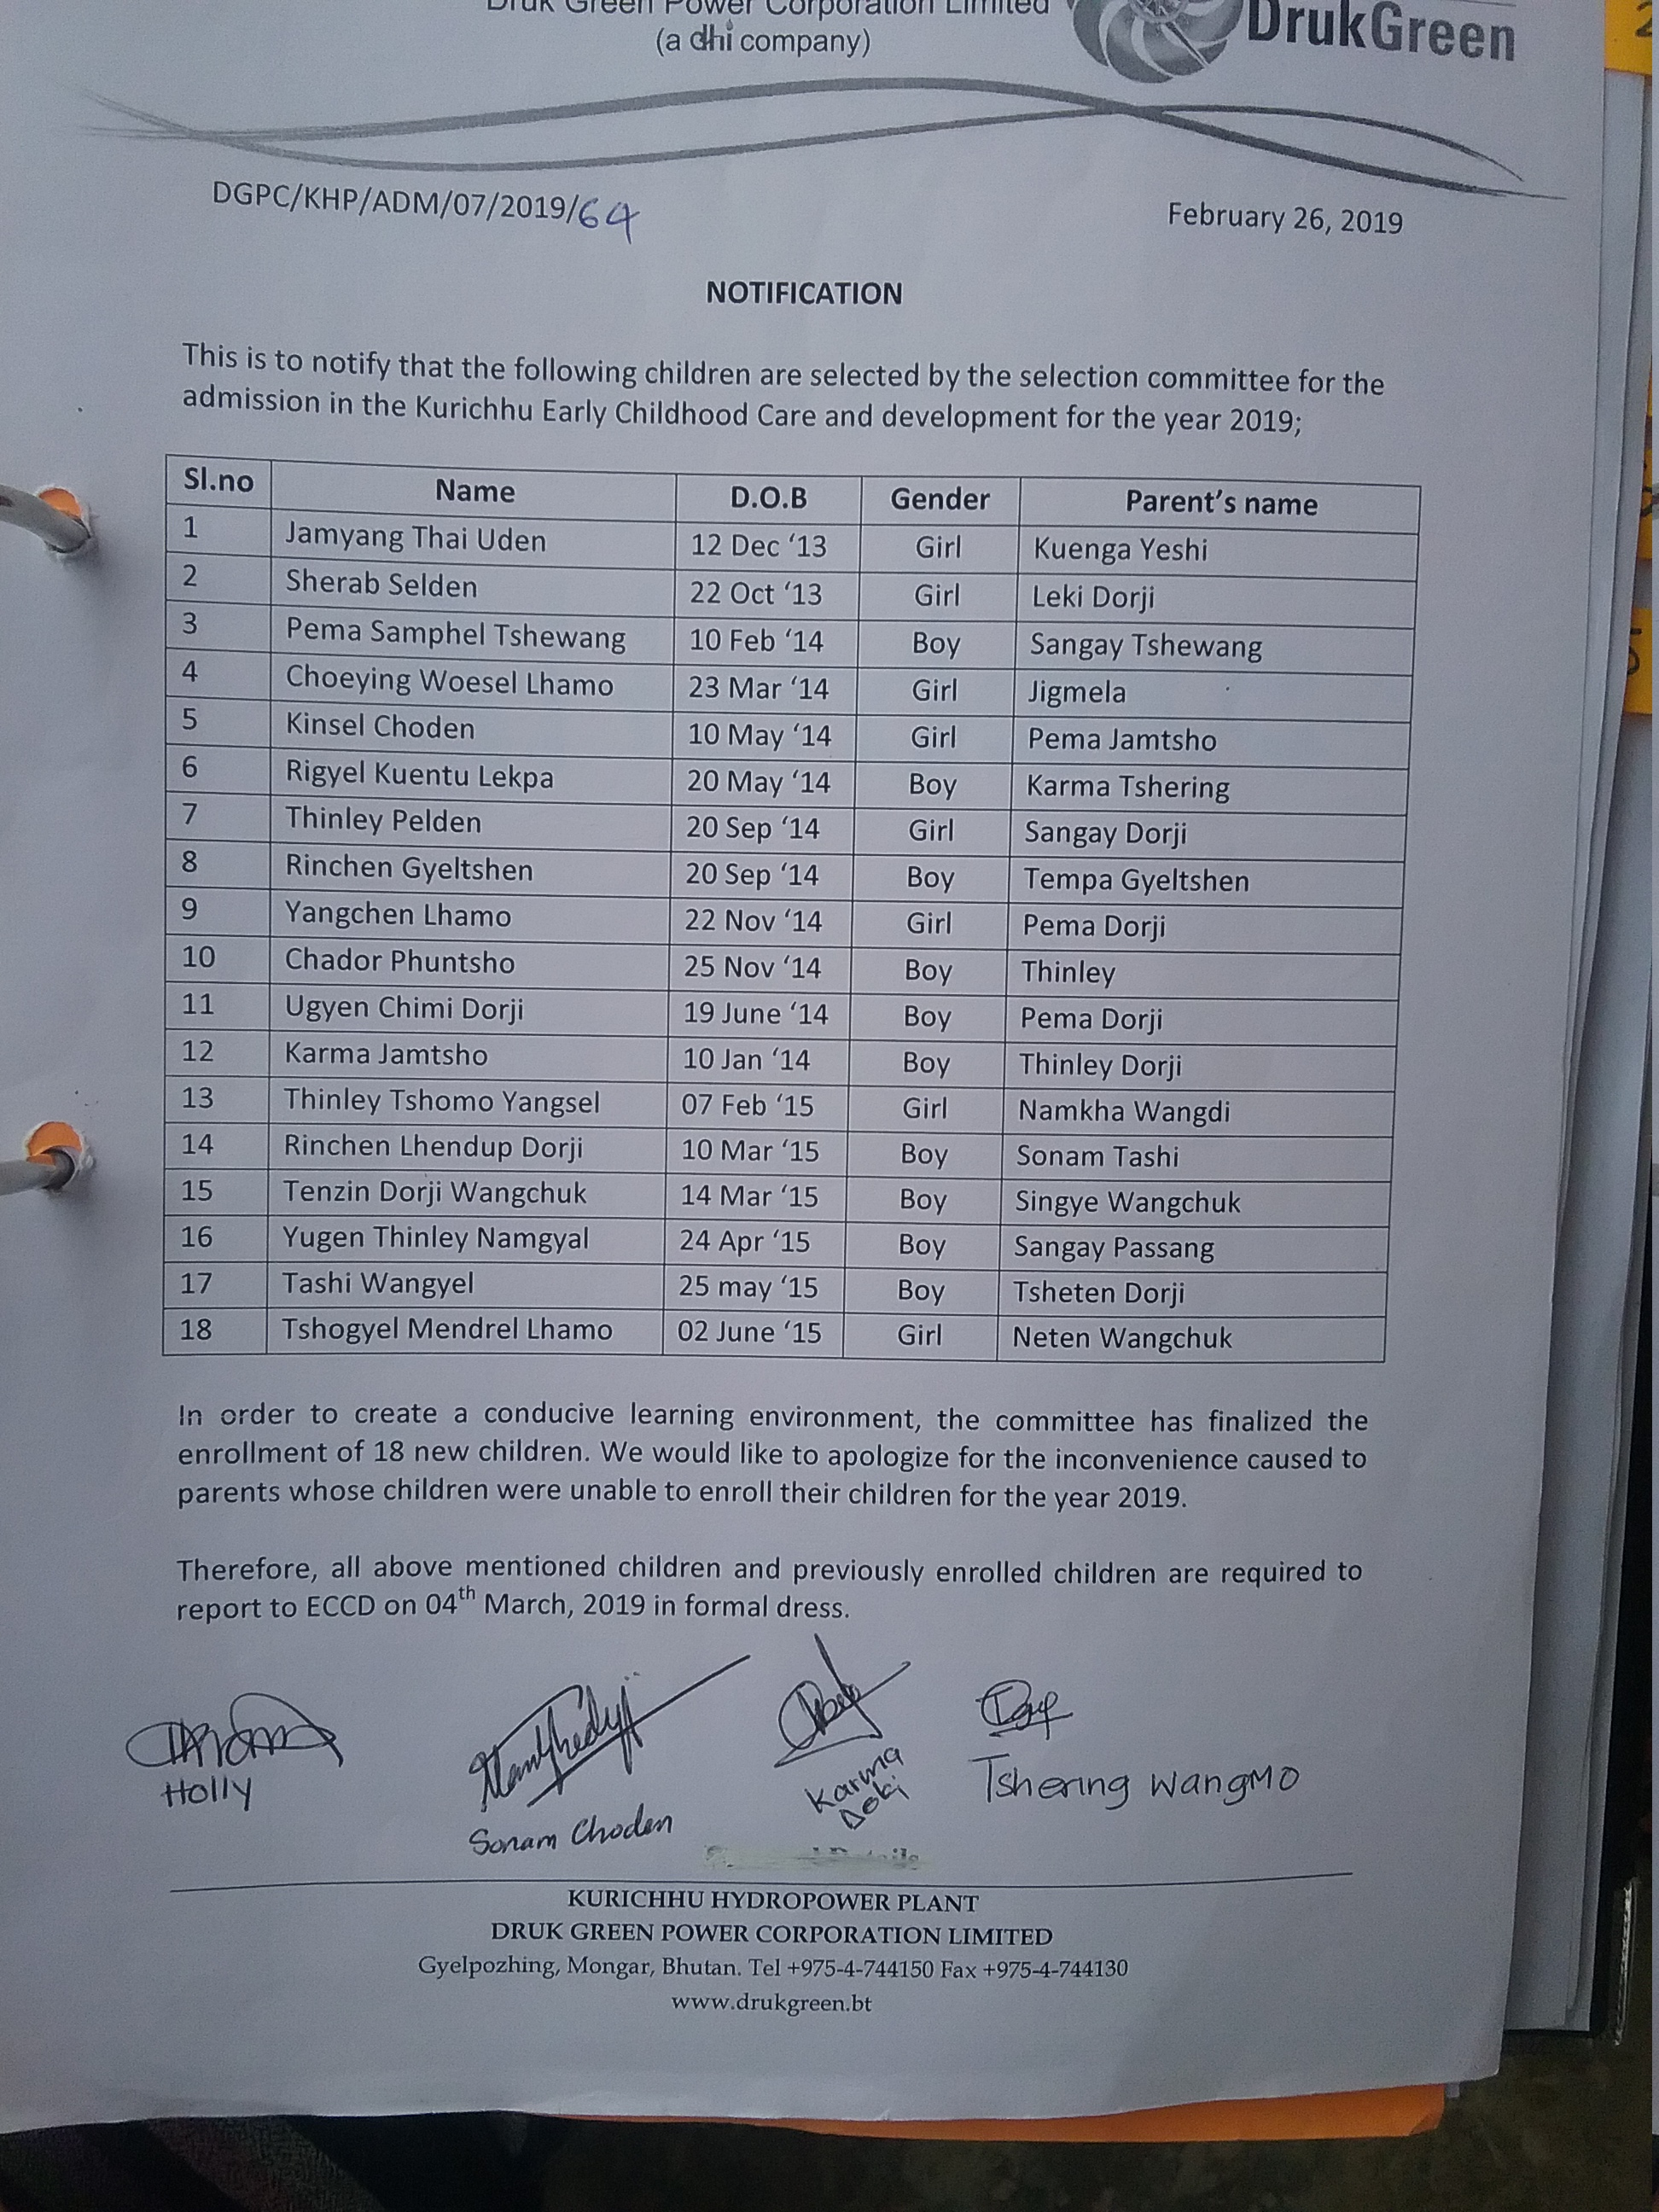
\includegraphics[scale=.2]{5}
		
		The record for attendance is also maintained in the same file.
		
		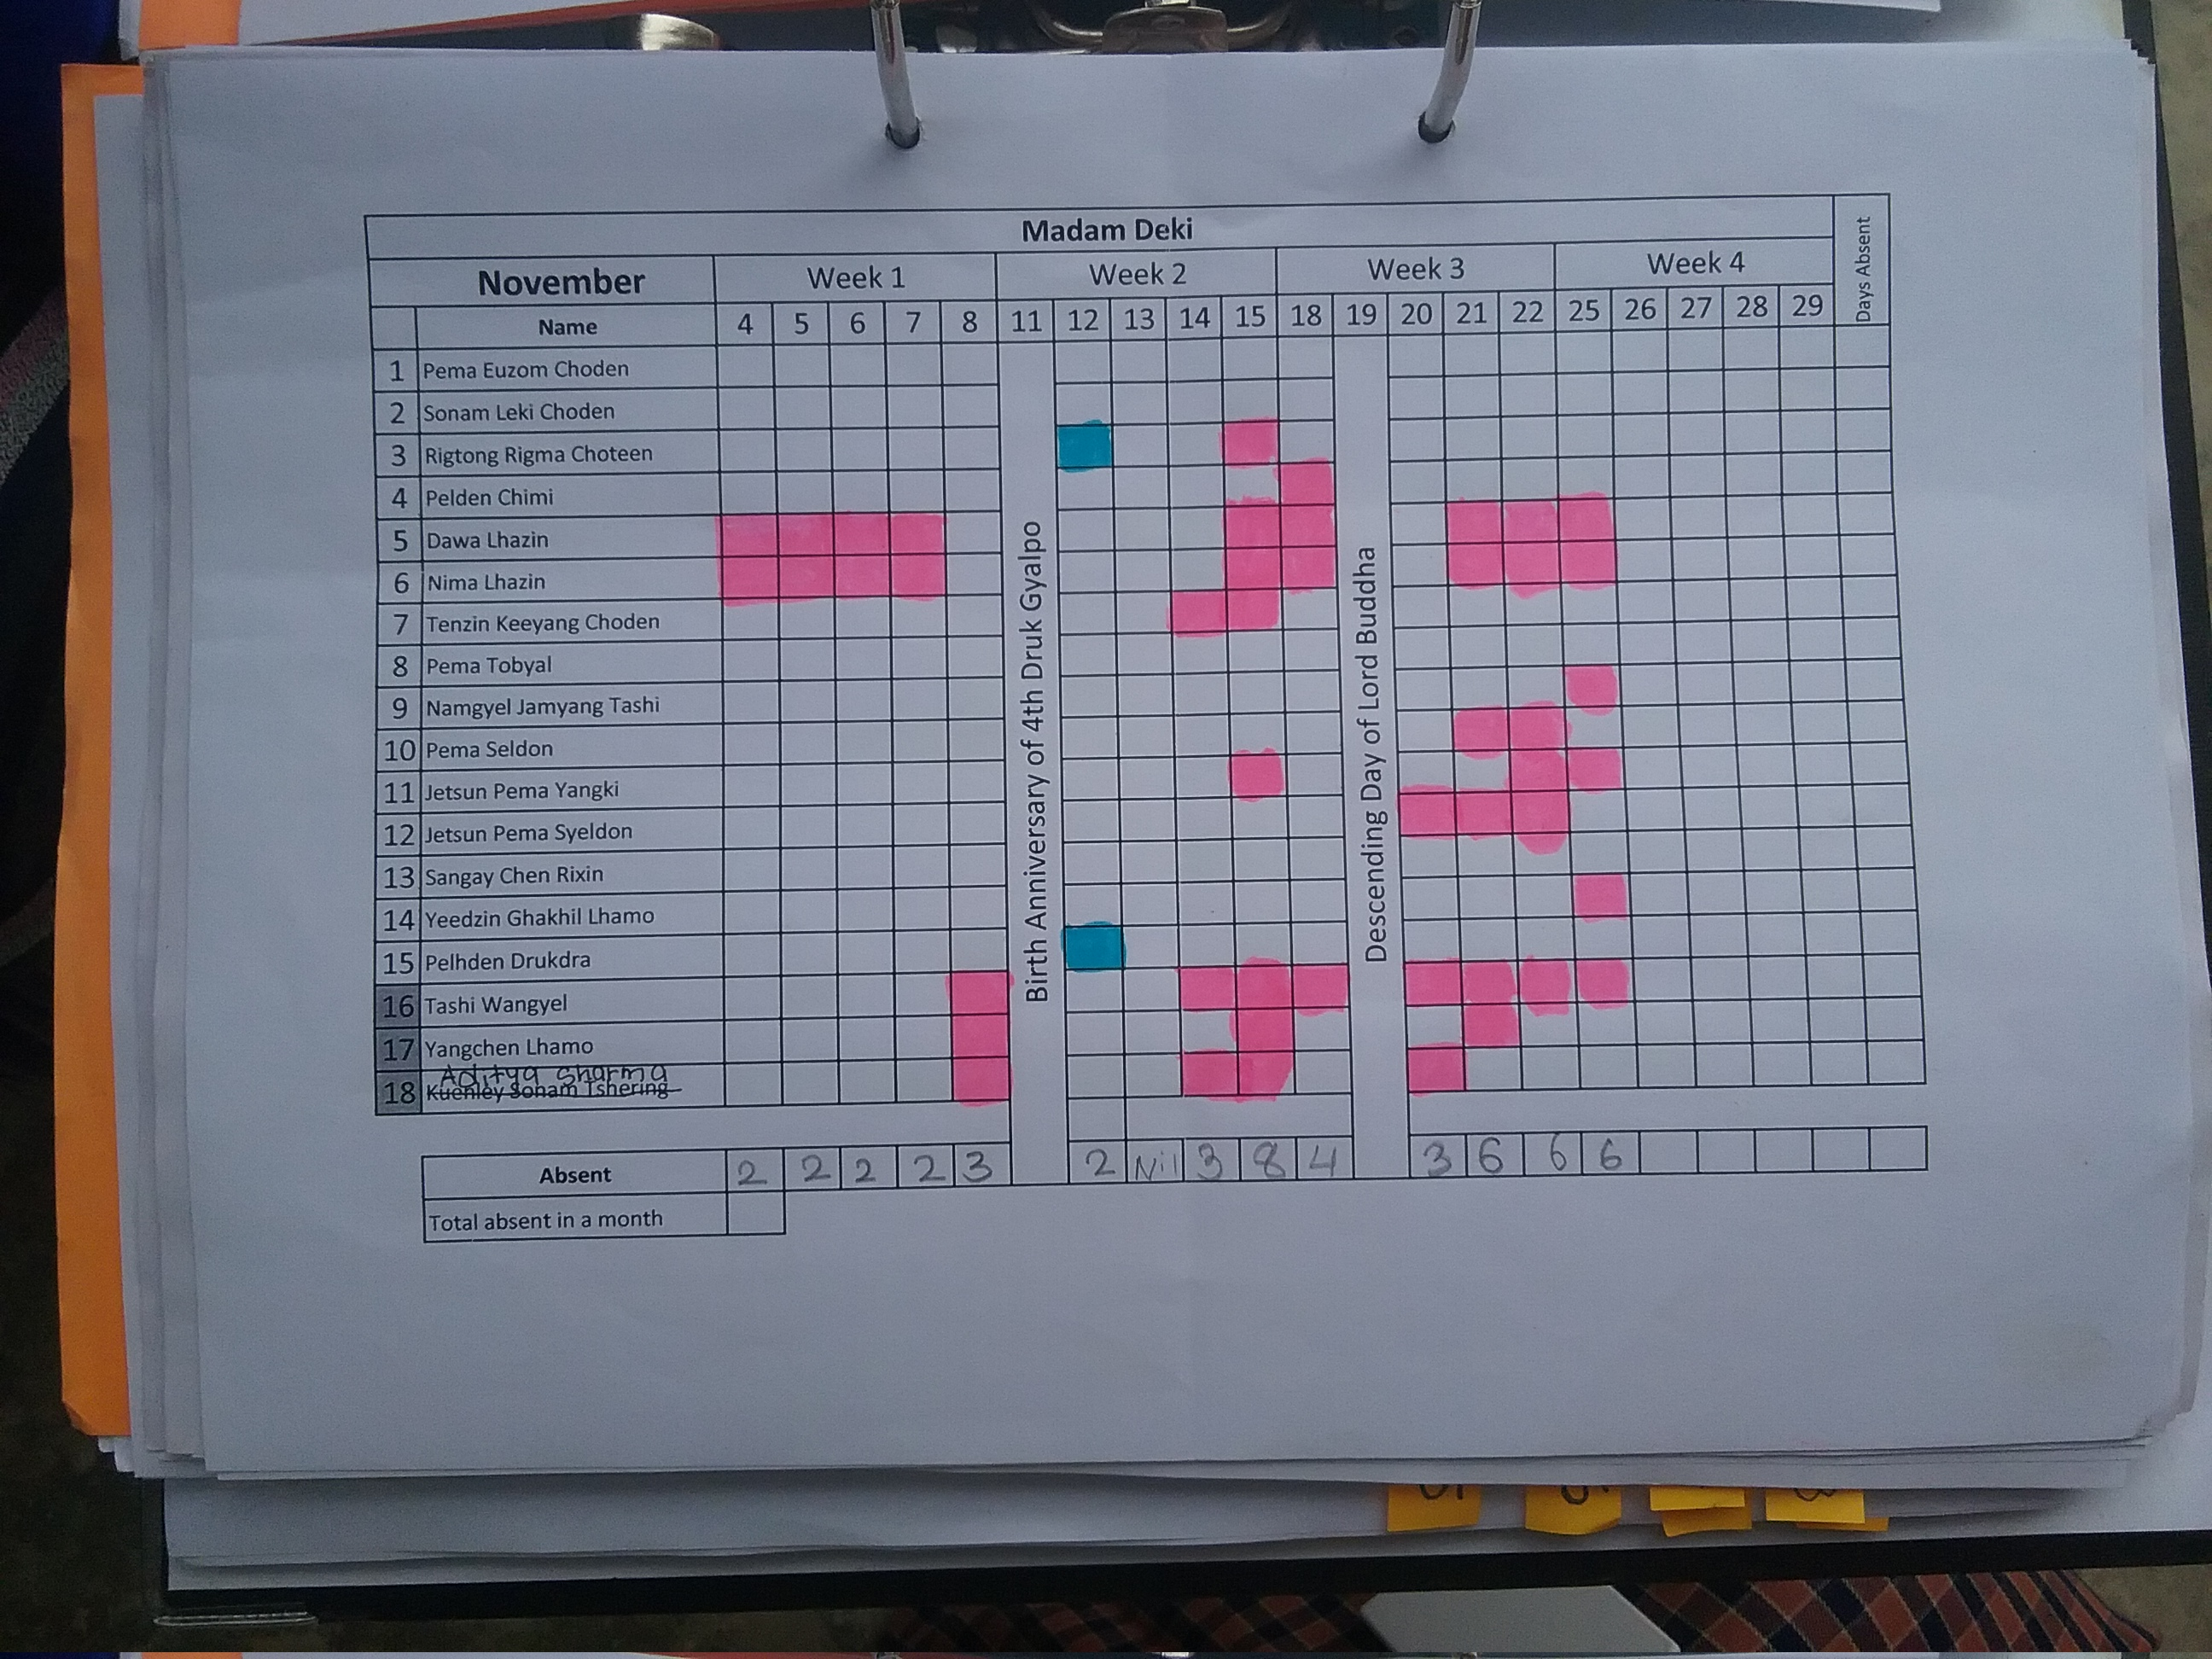
\includegraphics[scale=.2]{9}
		
		The information on the facilitator are kept in the paper file.
		
		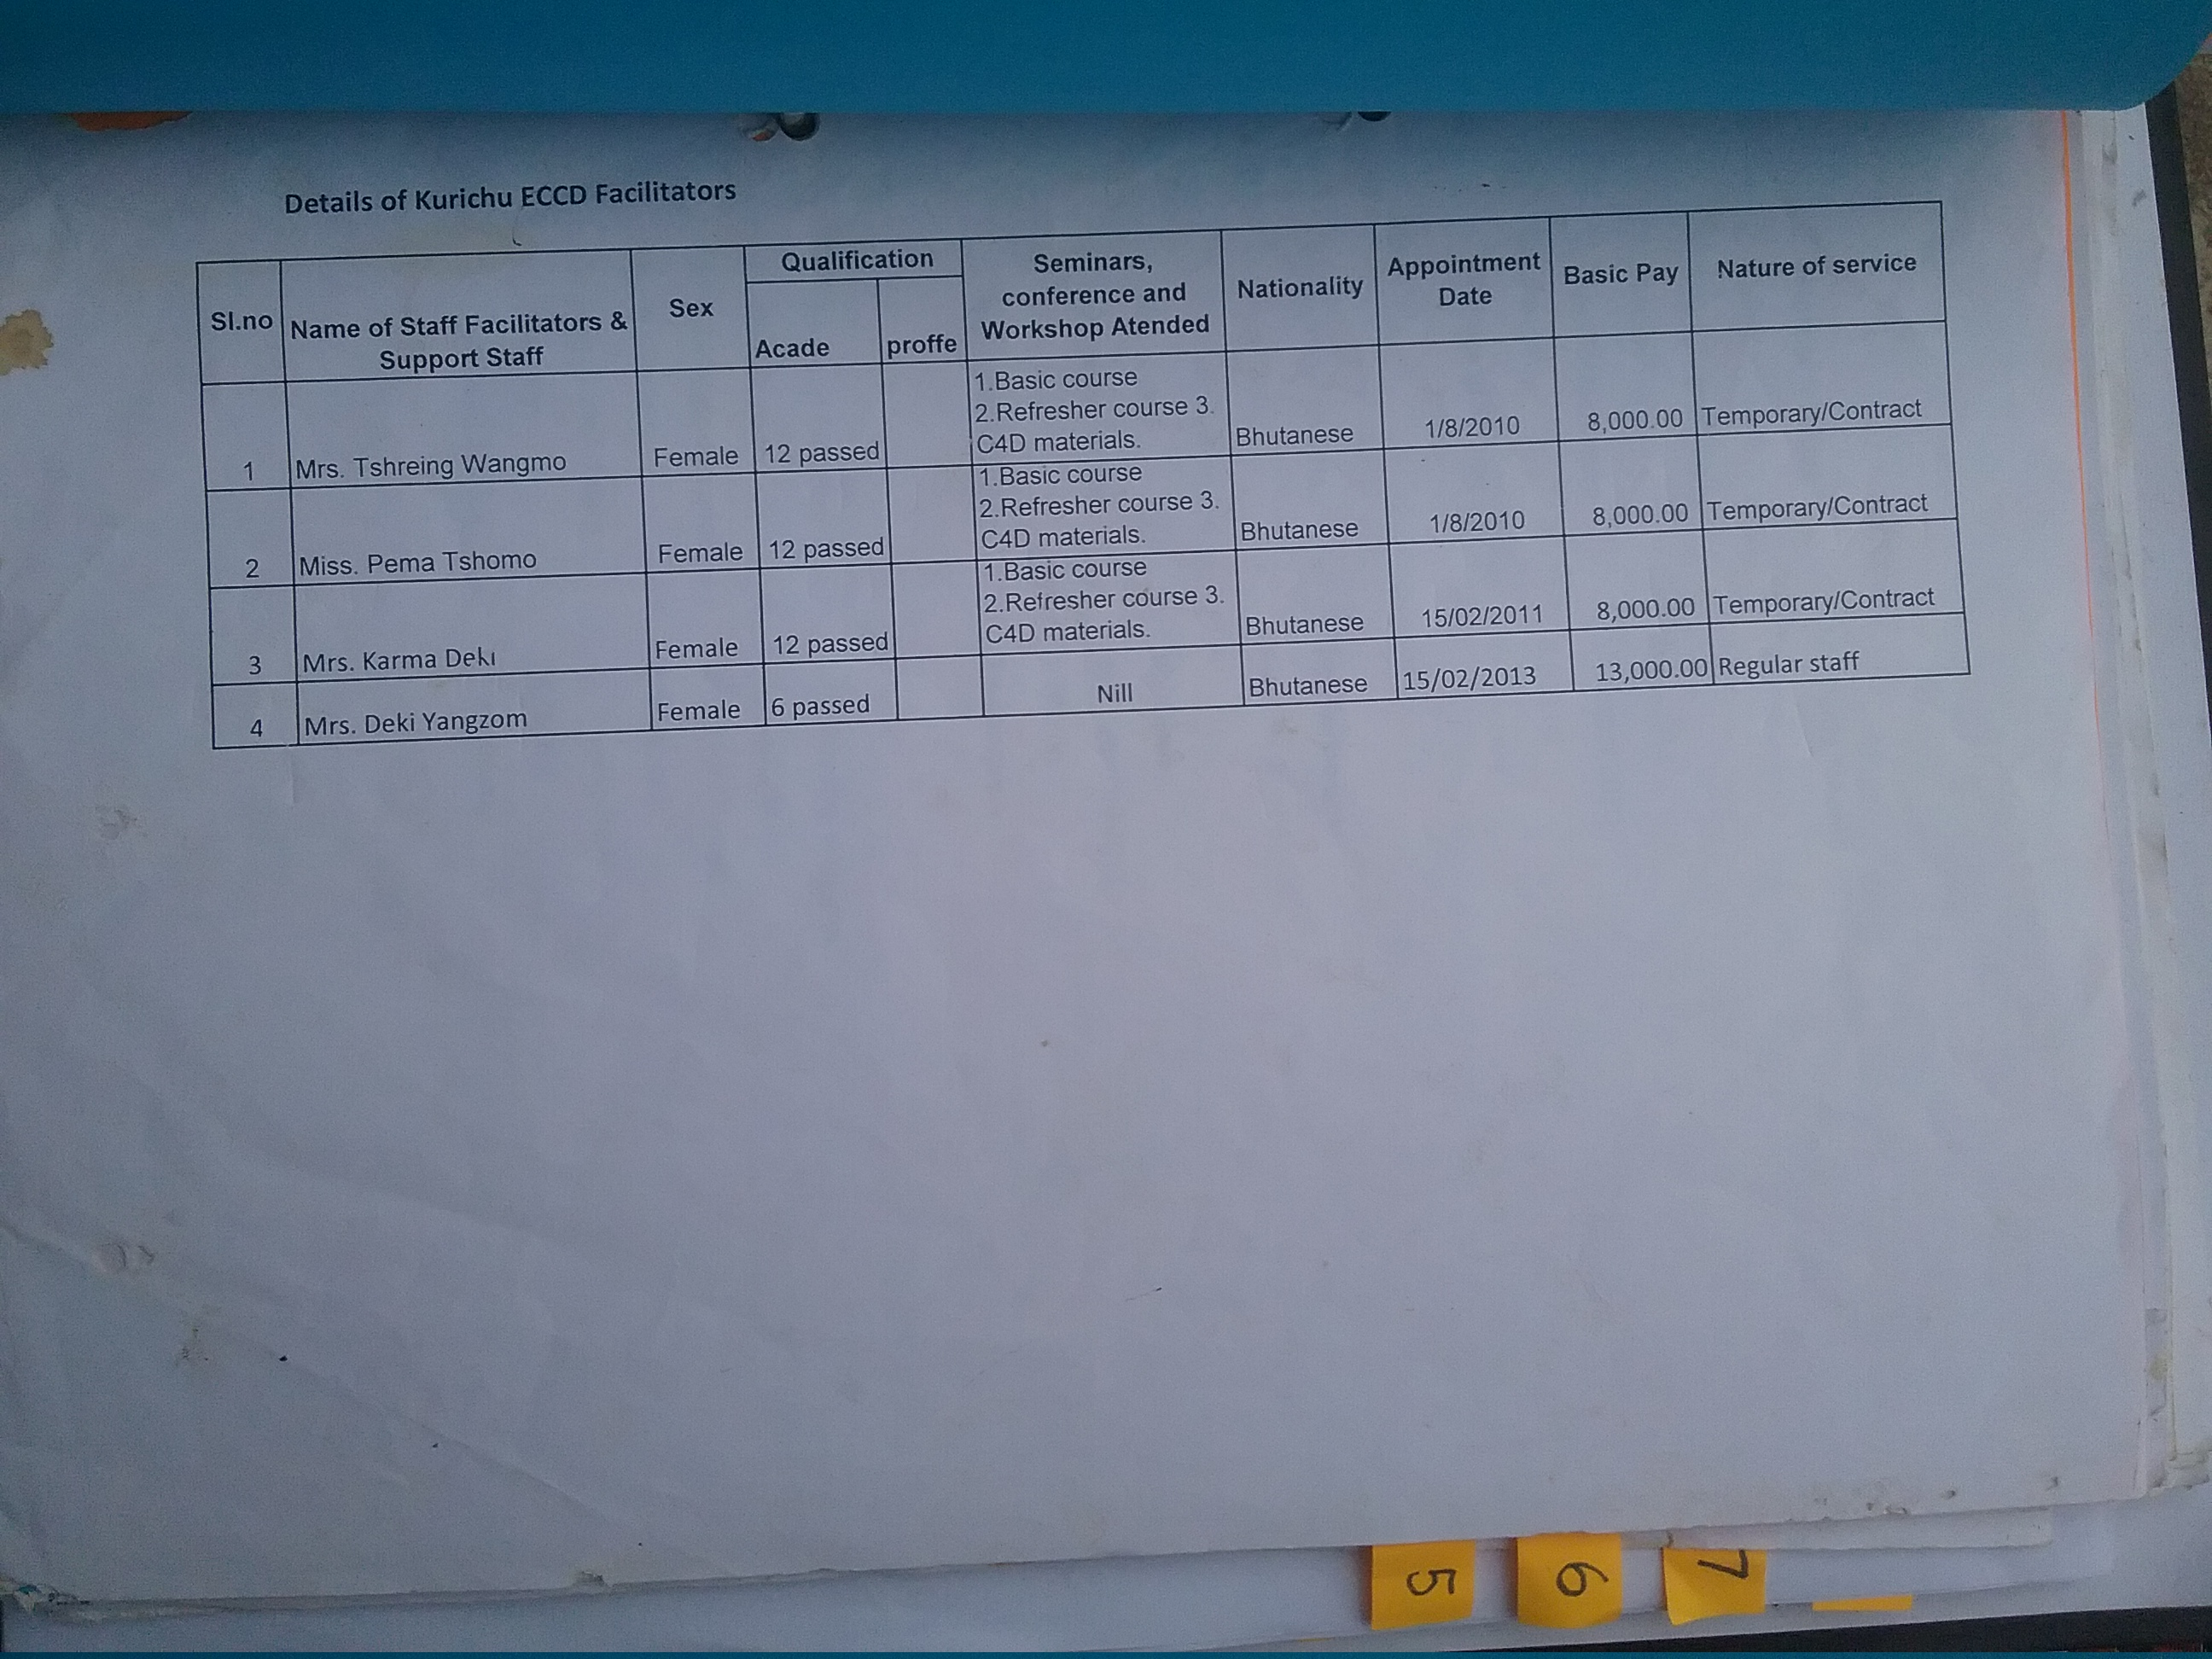
\includegraphics[scale=.2]{17}
	\end{itemize}
	
	
	\section{Expected ER Model}
	\begin{itemize}
		\item Entities
		\begin{itemize}
			\item Facilitator
			\item Children
			\item Guardian
			\item Workshop
		\end{itemize}
	

		\item Relationship among the Entities
		\begin{itemize}
			\item Facilitator cares Children
			\item Child has a Guardian
			\item Facilitator attends Workahop
		\end{itemize}
	\end{itemize}
	\section{Work Plan}
	
	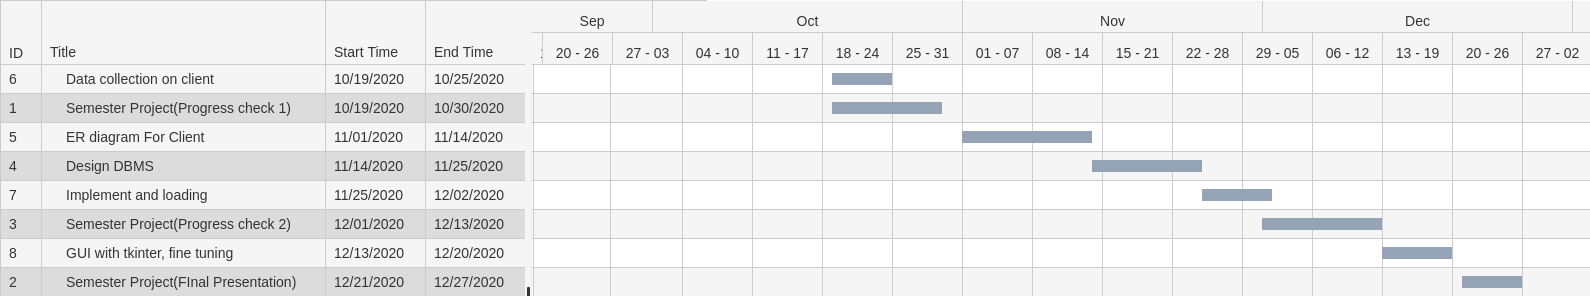
\includegraphics[scale=.3]{Gantt Chart}

	
\chapter{Database Design}
\section{ER model of ECCD}
	
	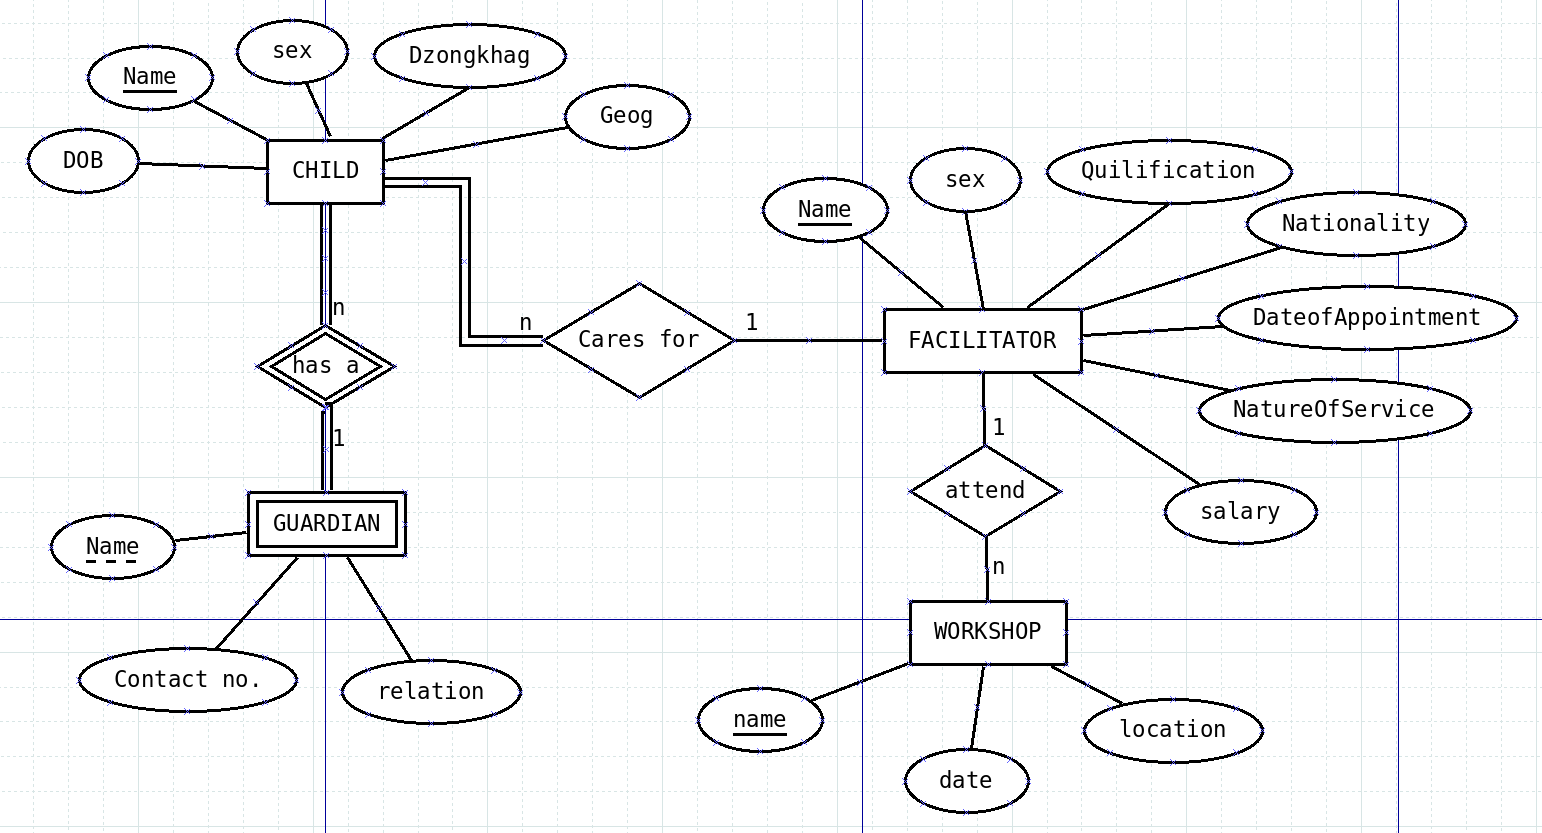
\includegraphics[scale=.3]{er}
	
\section{Logical Design}

	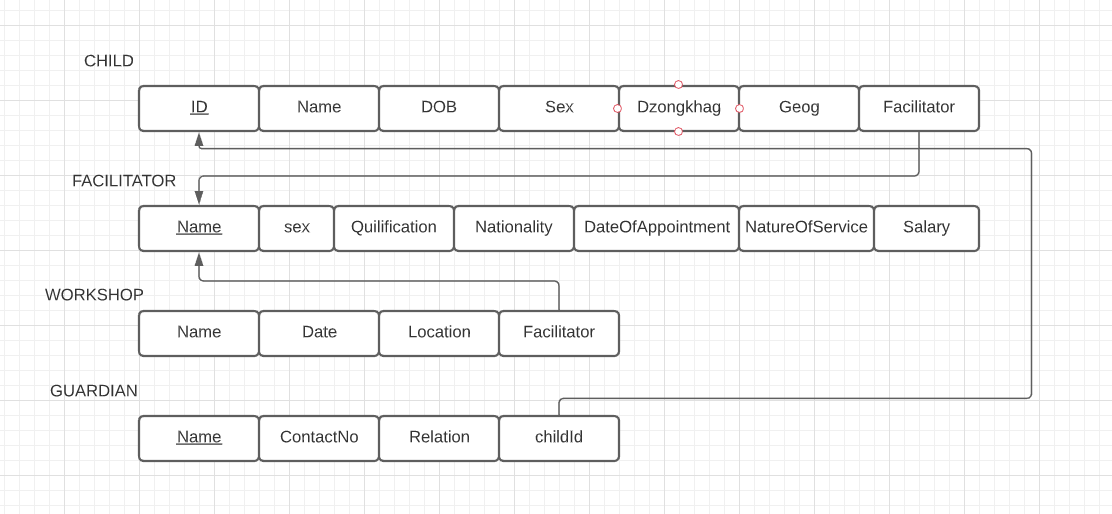
\includegraphics[width = \linewidth]{schema}


\chapter{Implementation}
	\section{Physical Design}
	
	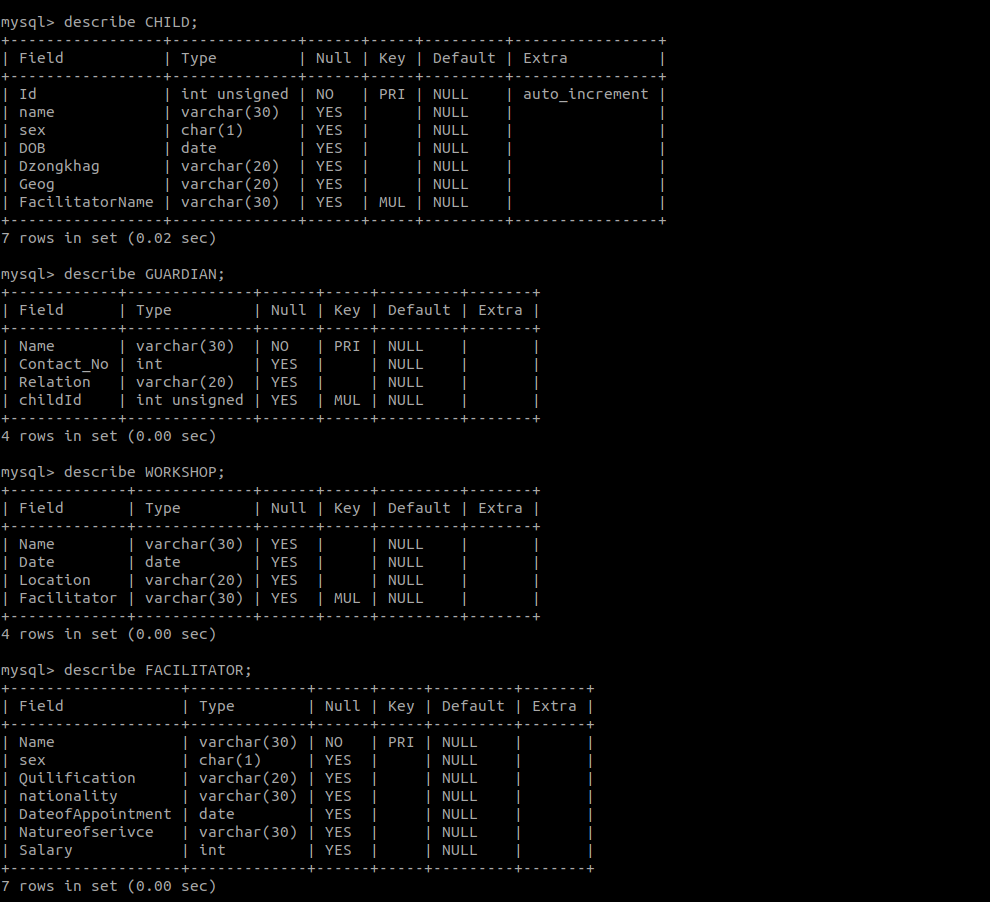
\includegraphics[width = \linewidth]{phy}
	Above tables are the real tables in the database.
		
	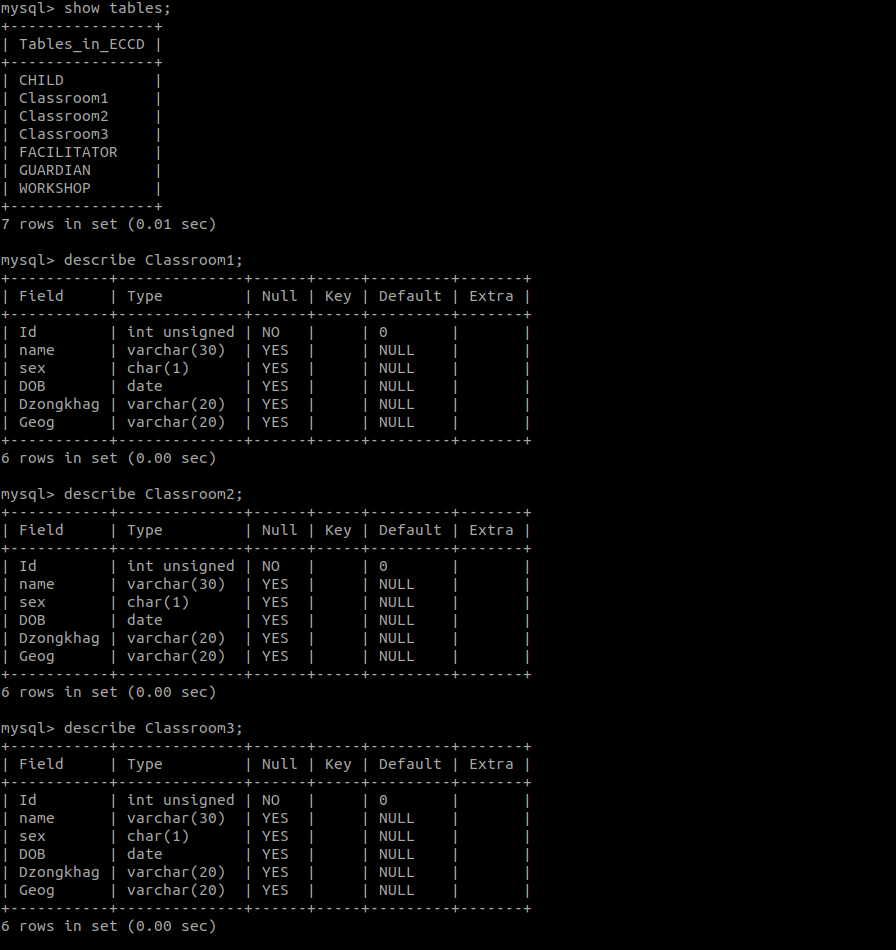
\includegraphics[width = \linewidth]{tab}
	Above colours are the views made from the child table.
	\section{Python Database Connectivity}
	
	\lstinputlisting[language=Octave]{Student.py}
	
	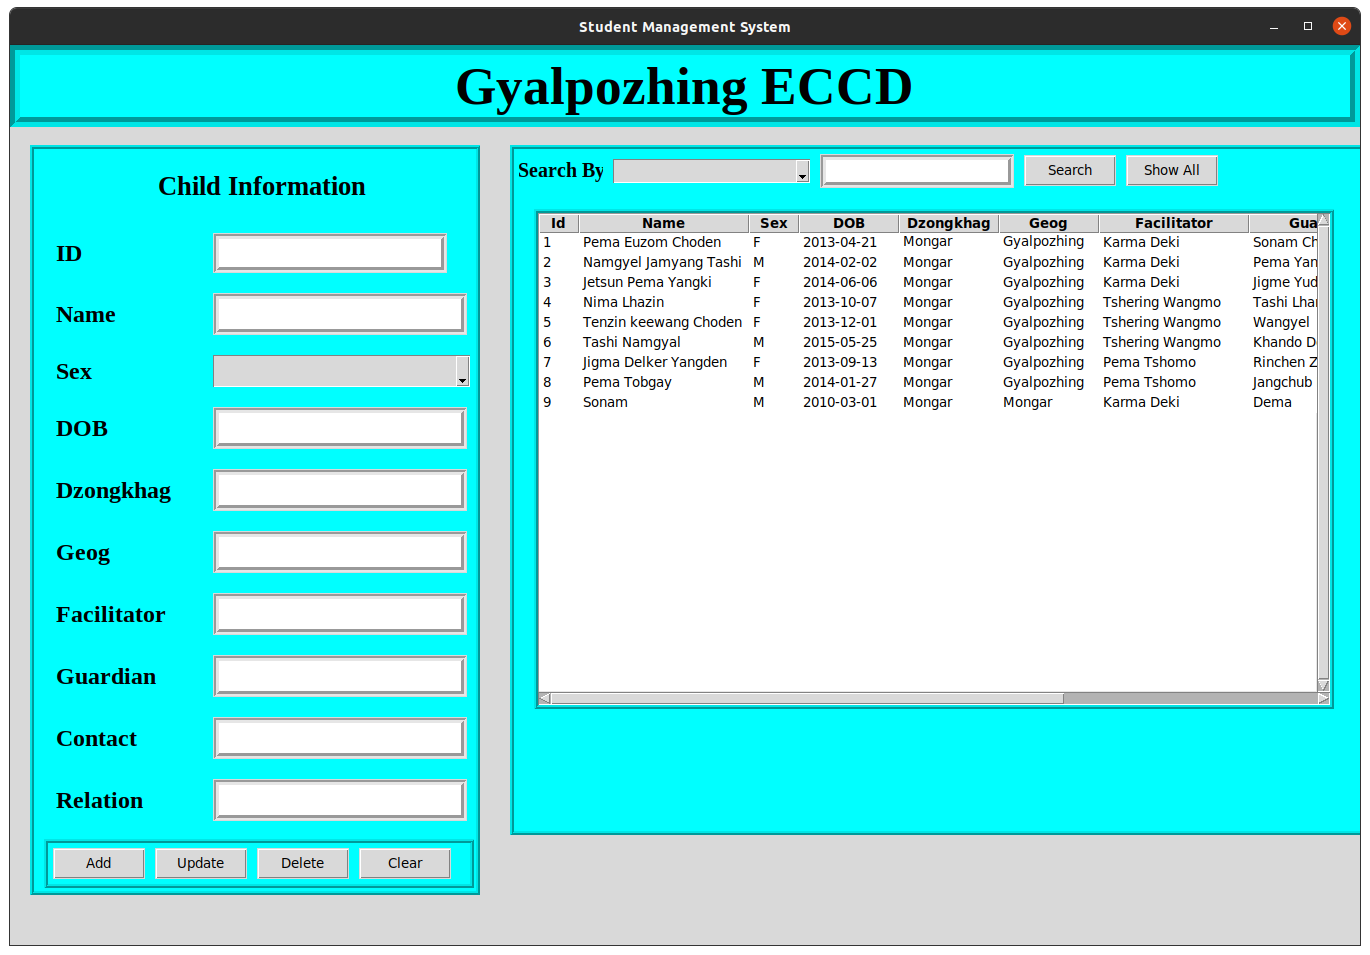
\includegraphics[width = \linewidth]{gui}
	GUI application to access the database
	
\chapter*{Conclusion}
	The ECCD database contains records for children, their guardian, the facilitators, and the workshops attended by the facilitators.\\From this project the members of the group has learned how to gather requirements for the database, desigh the logical and physical structure of the relations.\\Learned to use python to connect to mysql and create a GUI to access the database.\\ \\The python connectivity GUI application currently contains the GUI interaction for adding, updating, deleting records in the child table and the guardian table.\\We may further develop the GUI to be able to access and create changes in the facilitator table and the classroom views as well.  

\begin{thebibliography}{99}			 
	
	\bibitem{key1} Klein, B.(2020) Python Course, url: https://www.python-course.eu/python_tkinter.php
    
    \bibitem{key2} sharptutorial (2020) Student Entry Tkinter, url: https://www.sharptutorial.com/database-with-gui-python/
	
	\bibitem{key3} Chaitanya Singh(2020) Normalization in DBMS: 1NF, 2NF, 3NF and BCNF in Database, url: https://beginnersbook.com/2015/05/normalization-in-dbms/
		

\end{thebibliography}
	

\end{document}